% !TeX program = xelatex

% !TEX encoding = UTF-8 Unicode
%this is a very simple document using xepersian package

\documentclass{article}
\usepackage{tcolorbox,mdframed}
\usepackage{physics, amsmath, amsfonts, fixmath, geometry, tikz, pgf, multirow, hyperref, amsfonts,amssymb, mathtools, physics, xcolor, siunitx, subcaption,tcolorbox}
\usepackage{graphicx}
\usepackage{pifont}
\usepackage{xcolor}
\usepackage{fontspec}
\usepackage{xepersian}
\setdigitfont{XB Niloofar}
\settextfont[]{XB Niloofar}
\settextfont[Scale=1]{XB Niloofar}
\setdigitfont{XB Niloofar}

%\setlatintextfont{Linux Libertine}
\setlength{\textwidth}{17 cm}
\setlength{\evensidemargin}{1 cm}
\setlength{\oddsidemargin}{-0.7 cm}
\linespread{1.9}
\title{ سری اول تمرینات درس ریاضی‌فیزیک پیشرفته - دکتر کریمی‌پور
\\
\vspace{-1em}
خمینه‌ها - قسمت‌اول
}

\author{موعد تحویل پاسخ‌ها:
 سوم اردیبهشت سال ۱۴۰۳ - تا ساعت 59:23
 \\
 از طریق 
 \href{https://cw.sharif.edu/}{سامانه درس‌افزار}
\\
دانشکده فیزیک - دانشگاه صنعتی شریف
}\date{}

\newcommand{\pardev}[2]{
	\frac{\partial #1}{\partial #2}
}

\begin{document}
	%\romantoday
	\maketitle
	
	\def\lo{\longrightarrow}
	\def\endline{		{
			\vspace{-2.5em}
			\color{cyan}
			\begin{center} \linethickness{1mm}\line(1,0){500} \end{center}
	}}
\def\thinendline{		{
		\vspace{-2.5em}
		\color{purple}
		\begin{center} \linethickness{0.5mm}\line(1,0){500} \end{center}
}}

		\endline
		
		\noindent
		\textbf{سوال اول:}
		در فضای 
		$\mathbb{R}^n$
		شار زیر را در نظر بگیرید:
		\[
		\alpha(t) : \mathbf{x} \longmapsto t\mathbf{x}.
		\]
		میدان برداری وابسته به این شار را پیدا کنید.
		
		\endline
		
		\noindent
		\textbf{سوال دوم:}
		در فضای 
		$\mathbb{R}^2$
		 با مختصات موضعی 
		 $(x,y)$
		 میدان‌های برداری زیر را در نظر بگیرید:
		 \begin{equation*}
		 	\begin{aligned}
		 		X = x\pardev{}{x} - y\pardev{}{y},\quad\quad
		 		Y = x\pardev{}{y} + y\pardev{}{x},\quad\quad 
		 		Z = x^2\pardev{}{x} + y^2\pardev{}{y}. 
		 	\end{aligned}
		 \end{equation*}
		 الف) شارهای مربوط به این میدان‌های برداری را حساب کنید.
		 
		 \noindent
		 ب)جابه‌جاگرهای میدان‌های برداری فوق را بیابید.
		 
		 \noindent
		 ج) مشتقات لی زیر را حساب کنید:
		 \[
		 \mathcal{L}_XY,\quad \mathcal{L}_XZ, \quad \mathcal{L}_YZ
		 \]
		
		\endline
		
		
\noindent
\textbf{سوال سوم:}
در صفحه 
$\mathbb{R}^2$
نگاشت زیر را در نظر بگیرید:
\[
R: (x^1,x^2) \lo (x^1\cos\theta + x^2\sin\theta, -x^1\sin\theta + x^2\cos\theta)
\]
تحت این نگاشت حساب کنید که بردار 
$X = X^1 \pardev{}{x^1} + X^2\pardev{}{x^2}$
به چه برداری تبدیل می‌شود. 

\noindent
از نظری شهودی، رابطه بردار جدیدی که بدست آمده با بردار اولیه چیست؟ همین سوال را برای یک فرم دیفرانسیل نیز پاسخ دهید.

	\endline
				
		\noindent
		\textbf{سوال چهارم:}
		در فضای سه بعدی دکارتی تانسور زیر تعریف شده است:
		\[
		g = dx\otimes dx + dy\otimes dy + dz\otimes dz
		\]
		تحت نگاشت
		\[
		x=r\sin\theta\cos\phi,\quad y = r\sin\theta\sin\phi,\quad z=r\cos\theta,
		\]
		تبدیل تانسور فوق را بدست آورید. به عبارت دیگر 
		\lr{Pullback}
		تانسور 
		$g$ را بدست آورید. 
		به چه چیزی می‌رسید؟
		
		\noindent
		این کار را برای فرم دیفرانسیل زیر نیز انجام دهید:
		\[
		\omega = dx \wedge dy\wedge dz.
		\]
		\vspace{-4em}
	\endline
	\vspace{-2em}
				
		\noindent
		\textbf{سوال پنجم:}
در فضای 
$\mathbb{R}^3$
میدان‌های برداری زیر را در نظر بگیرید:
\[
L_x = y\pardev{}{z} - z\pardev{}{x},\quad\quad
L_y = z\pardev{}{x}- x\pardev{}{z},\quad\quad
L_z = x\pardev{}{y}  - y\pardev{}{z}.
\]

\noindent
الف)نشان دهید که این سه میدان برداری تحت حابه‌جاگر یک جبربسته تشکیل می‌دهند. شار مربوط به هر میدان برداری را بدست آورید. نتیجه را از نظر شهودی تعبیر کنید.

\noindent
ب) به میدان‌های قسمت قبل میدان‌های زیر را اضافه کنید:
\[
P_x = \pardev{}{x},\quad\quad
P_y = \pardev{}{y} , \quad\quad
P_z = \pardev{}{z}.
\]
نشان دهید که مجموعه‌ی میدان‌های $L_i$ و $P_j$ تحت جابه‌جاگر یک جبر بسته تشکیل می‌دهند.

		\endline
		
\textbf{سوال ششم:}
روابط زیر را برای میدان‌های برداری و مشتق لی ثابت کنید.
\begin{equation*}
	\begin{aligned}
		\mathcal{L}_{fX}Y &= f[X,Y]- Y[f]X, \\
		\mathcal{L}_X(fY) &= f[X,Y] + X[f]Y.
	\end{aligned}
\end{equation*}
که در آن 
$X,Y \in \mathcal{H}(M)$ و
$f \in \mathcal{C}^\infty(M)$
به ترتیب میدان‌های بردای و تابع هموار روی خمینه $M$ هستند.
		
	
	\endline
	\noindent
	\textbf{تمرین‌های کلاسی:}
	
	\noindent
	\textbf{الف)} با نگاشت 
	\lr{Pushforward}
	 (گاه به آن نگاشت دیفرانسیل می‌گویند و با $d\varphi$ نشان می‌دهند.) در کلاس آشنا شدید. اگر نگاشت $\varphi$ بین دو خمینه هموار موجود باشد، آنگاه نگاشت \lr{Pushforward} وظیفه‌ی نگاشتن کلاف‌های مماس را بین این دو خمینه به عهده می‌گیرد.
	 \[
	 \varphi^* : T_p M \longmapsto T_{\varphi(p)}N
	 \]
	 
	 \begin{figure}[h]
	 	\centering
	 	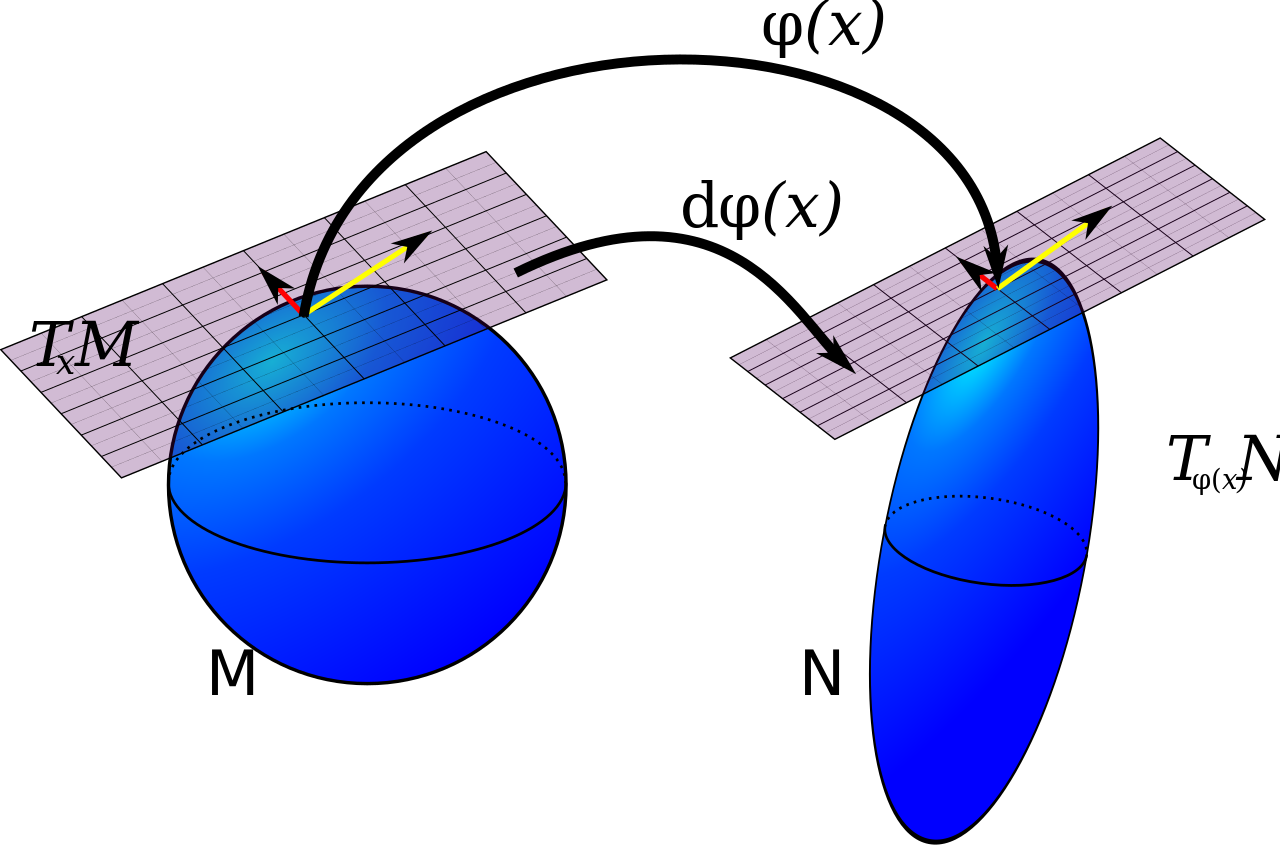
\includegraphics[width=30em]{1.png}
	 	\caption{نگاشت بین خمینه‌های هموار و نگاشت \lr{Pushforward}}
	 	\label{fig1}
	 \end{figure}
گزاره‌هایی را که در کلاس به عنوان تمرین به شما واگذار شده است، حل کنید.
\begin{enumerate}
	\item ثابت کنید
	$\varphi^*(X)$
	یک بردار است.
	\item با کمک تعریف ذاتی 
	\[
	\Big(\underbrace{\varphi^*(\overbrace{X}^{\in T_pM})}_{\in T_{\varphi(p)}N}\Big)[\overbrace{f}^{\in C^\infty (N)}]  := X(\underbrace{f\circ \varphi}_{\in \mathcal{C^\infty}(M)})
	\]
	مولفه‌های $\varphi^*(X)$ در 
	$T_{\varphi(p)}N$
	را حاصل کنید.
	\item خطی بودن نگاشت \lr{Pushforward} را نشان دهید.
\end{enumerate}
\thinendline

\noindent
\textbf{ب)}
تمرین‌قبل را برای نگاشت 
\lr{Pullback}
انجام دهید.

\noindent
نگاشت \lr{Pullback}، هم‌بردارها و فرم‌های فضای مقصد را به هم‌بردارها و فرمهای فضای مبدا می‌نگارد:
\[
\Big(\overbrace{\varphi_* (\underbrace{\omega}_{\in T^*_{\varphi(p) }N})}^{\in T^*_p M} \Big) [\overbrace{X}^{\in T_p M}] := \omega\big(
\underbrace{\varphi^*(X)}_{\in T_{\varphi(p)}N}
\big)
\]
\thinendline

\noindent
\textbf{ج)}
رابطه‌ی زیر برای براکت لی را هم ثابت کنید
\footnote{ممنون از آقای پوربهرامی بابت تذکر نکته به‌جایشان.}
.
\[
\varphi^*[X,Y] = [\varphi^*X,\varphi^*Y]
\]
\end{document}



